\documentclass[a4paper]{scrreprt}

\usepackage[german]{babel}
\usepackage[utf8]{inputenc}
\usepackage{hyperref}
\usepackage[bottom=10em, top=5em]{geometry}
\usepackage{amsmath}
\usepackage[pdftex]{graphicx}
\usepackage{booktabs, array}
\usepackage{eurosym}
\usepackage{float}

\usepackage{chngcntr}
\counterwithout{figure}{chapter}
\renewcommand{\figurename}{Abbildung}

\newcommand{\HRule}{\rule{\linewidth}{0.5mm}}

\begin{document}

\author{S. Biereigel, R. Winkler, M. Fugmann, J. Yin}
\title{Laborbuch Mikrorechnerentwurf}

\begin{titlepage}
\vspace*{\fill}
\begin{center}
	\textsc{\LARGE Ernst-Abbe-Hochschule Jena} \\ [1.5cm]

	\textsc{\Large Projekt Mikrorechnerentwurf} \\ [0.5cm]

	\HRule \\ [0.3cm]
	{\LARGE AsuroMote}\\	[0.3cm]
	{\Large Entwicklung einer Roboterfernsteuerung }
	\HRule \\ [1 cm]

	\begin{minipage}{0.4\textwidth}
		\begin{flushleft} \large
			\emph{Gruppenmitglieder:}\\
			Stefan \textsc{Biereigel}\\
			Rene \textsc{Winkler}\\
			Mathias \textsc{Fugmann}\\
			Junlong \textsc{Yin}\\
		\end{flushleft}
	\end{minipage}
	\begin{minipage}{0.4\textwidth}
		\begin{flushright} \large
			\emph{Betreuer:}\\
			Burkart \textsc{Voß}\\
		\end{flushright}
	\end{minipage}

\end{center}
\vspace*{\fill}
\end{titlepage}


\tableofcontents
\pagebreak

\chapter{Treffen am 29.09.2014}
\section{Anwesende Personen}
\begin{itemize}
	\item Stefan Biereigel
	\item Rene Winkler
	\item Mathias Fugmann
	\item Junlong Yin
\end{itemize}

\section{Besprochen bzw. Bearbeitet}
\begin{itemize}
	\item Kundengespräch mit Herrn Voß
		\begin{itemize}
			\item Aufgabenstellung erhalten
			\item Kostenrahmen definiert
		\end{itemize}
	\item Erarbeitung der Spezifikation
\end{itemize}

\section{Problemstellung des Kunden}
\begin{itemize}
	\item Übertragung von Daten zum ASURO zu störanfällig (andere ASURO, Umwelteinflüsse)
	\begin{itemize}
		\item Diskussion: Kam uns nicht sehr störanfällig vor
		\item Fehlererkennung und -korrektur ist bereits vorhanden
		\item könnte man auch weiternutzen (über anderes Übertragungsmedium?)
	\end{itemize}
	\item Fernsteuerung für den ASURO fehlt
	\begin{itemize}
		\item erste Idee: WiiMote-ähnliche Steuerung wäre ansprechend
	\end{itemize}
\end{itemize}


\section{Spezifikation}
Legende: F = Forderung, W = Wunsch
\begin{itemize}
	\item Hauptanforderungen
	\begin{itemize}
		\item (F) Steuerung des ASURO über min. eine Eingabemöglichkeit
		\item (F) Programmierung des ASURO (Flashen) über eine Schnitstelle	
	\end{itemize}

\item Leistungsfähigkeit (Performance)
	\begin{itemize}
		\item (F) Steuerung aller Bewegungsrichtungen
		\item (F) Kommunikation mit ASURO fehlertolerant / nicht störanfällig
		\item (F) Kommunikationsreichweite minimum fünf Meter
		\item (W) Kommunikation in gesamtem Raum möglich
	\end{itemize}
\item Energieversorgung
	\begin{itemize}
		\item (F) Kabellose Stromversorgung
		\item (W) Akkus im Gerät aufladbar
	\end{itemize}
\item Geometrie
	\begin{itemize}
		\item (F) Handgerät, zweihändige Bedienung
	\end{itemize}
\item Budget
	\begin{itemize}
		\item (F) Leistungsaufnahme: Gerätelaufzeit mindestens eine Stunde Dauerbetrieb
	\end{itemize}
	\begin{itemize}
		\item (F) Gewicht weniger als 500 Gramm
	\end{itemize}
	\begin{itemize}
		\item (F) Kosten maximal \EUR{50} exklusive STM32F4 Discovery Board
	\end{itemize}
	\begin{itemize}
		\item (F) Entwicklungs- und Herstellungszeit: Auslieferung spätestens 12. Semesterwoche im SS 2015
	\end{itemize}
\item Herstellungsprozess
	\begin{itemize}
		\item Elektronik in Eigenarbeit herstellen, Software selbst implementieren
	\end{itemize}
\item Standards
	\begin{itemize}
		\item (F) Einhaltung von in Deutschland gültigen, für den Betrieb notwendigen
	 Standards
	\end{itemize}
\item Sicherheit
	\begin{itemize}
		\item (F) keine gesundheitliche Gefährdung von Personen durch das Gerät
	\end{itemize}
\item Ergonomie
	\begin{itemize}
		\item (W) einfache Bedienbarkeit
		\item (W) ansprechendes Aussehen
		\item (W) ergonomische Handhabung
	\end{itemize}
\end{itemize}
\chapter{Treffen am 13.10.2014}
\section{Anwesende Personen}
\begin{itemize}
	\item Rene Winkler
	\item Mathias Fugmann
	\item Junlong Yin
\end{itemize}

\section{Besprochen bzw. Bearbeitet}
\begin{itemize}
	\item Design-Schritt 2 begonnen
	\item Erstellung der Konzeptskizzen für drei Varianten
\end{itemize}

\section{Ausarbeitung von drei Konzepten}
\subsection{Konzept Blau}
Zu sehen in \autoref{fig:blau_v1}.
\begin{itemize}
	\item soll einfache Bedienung ermöglichen
	\item Benutzung eines 4-Wege-Analogjoysticks zur Handsteuerung
	\begin{itemize}
		\item Beschaffbarkeit eventuell ein Problem!
	\end{itemize}
	\item ein günstiges LCD könnte Verwendung finden und alle interessanten 	Informationen anzeigen
	\item hoher Aufwand an Bluetooth-Modulen (3 Stück) - Kostenfaktor!
\end{itemize}

\subsection{Konzept Grün}
Zu sehen in \autoref{fig:gruen_v1}.
\begin{itemize}
	\item benutzt günstigeres Funkmodul zur Asuro-Kommunikation
	\item Verbindung zum PC kann entweder am Asuro oder an der Fernsteuerung erfolgen - flexibel
	\begin{itemize}
		\item Akku beider Geräte kann direkt per USB geladen werden - großer Vorteil!
	\end{itemize}
	\item Konzept kann optional die Neigungssensoren zur Steuerung benutzen, weil D-Pad eher eingeschränkt
	\begin{itemize}
		\item neue Darstellungsmöglichkeiten auf Display - könnte dann ein größeres Dot-Matrix-Display sein
	\end{itemize}
\end{itemize}

\subsection{Konzept Rot}
Zu sehen in \autoref{fig:rot_v1}.
\begin{itemize}
	\item Design verwendet zwei BT-Module, sowie die USB-Verbindung
	\begin{itemize}
		\item gutes User-Handling
	\end{itemize}
	\item Neigungssensoren sind einzige Steuerungsmöglichkeit
	\begin{itemize}
		\item man könnte Buttons evtl. durch ein Touchscreen ersetzen
		\item keine beweglichen Teile (günstig!)
		\item Touchscreen evtl. teurer
	\end{itemize}
	\item Herstellung für nicht-standard-Gehäuseform evtl. 3D-Drucker möglich!
\end{itemize}

\chapter{Treffen am 27.10.2014}
\section{Anwesende Personen}
\begin{itemize}
	\item Stefan Biereigel
	\item Rene Winkler
	\item Mathias Fugmann
	\item Junlong Yin
\end{itemize}

\section{Besprochen bzw. Bearbeitet}
\begin{itemize}
	\item Design-Schritt 2
	\begin{itemize}
		\item Überarbeitung der Konzepte, rückblickende Diskussion
		\item siehe \autoref{fig:blau_v2}, \autoref{fig:gruen_v2}, \autoref{fig:rot_v2}.
		\item Feedback zum Laborbuch erhalten, rückblickende Überarbeitung, hinzufügen von Diskussionspunkten
	\end{itemize}
	\item Beginn der Bearbeitung von Design-Schritt 3
	\item Herausarbeiten von Themen zur näheren Behandlung im Seminar
	\begin{itemize}
		\item Beschleunigungssensoren (Ansteuerung, Auswertung)
		\item AD-Wandler im STM32F4
		\item SPI- und UART-Schnittstellen
		\item Interrupts im STM32F4
		\item LC-Displays (Ansteuerung, Datenformat, ...)
	\end{itemize}
\end{itemize}

\section{Entscheidungskriterien zur Beurteilung der Konzepte}
\begin{itemize}
	\item Preis
	\item Bedienbarkeit
	\item Komplexität
	\item Ähstetik
	\item Funktionsumfang
	\item Zuverlässigkeit
	\item Beschaffbarkeit der Teile
\end{itemize}
\chapter{Treffen am 3.11.2014}
\section{Anwesende Personen}
\begin{itemize}
	\item Stefan Biereigel
	\item Rene Winkler
	\item Mathias Fugmann
	\item Junlong Yin
\end{itemize}

\section{Besprochen bzw. Bearbeitet}
Weil es für das fertige Produkt mit großer Wahrscheinlichkeit benötigt wird, ein SPI-Interface am STM32F4 und den Beschleunigungssensor auf dem Discovery-Board anzusteuern, entschieden wir uns für die Entwicklung eines Testmoduls für ebendiese Aufgaben. Als Ziel soll ein kompaktes Modul mit dokumentierten Schnittstellen sein.

Verantwortlich für die Kodierung ist Rene Winkler, der Rest der Gruppe beschäftigt sich aber ebenfalls mit der notwendigen Theorie. Eine abschließende Präsentation der Ergebnisse vor den anderen Gruppenmitglieden wurde angedacht.

Der Rest des Praktikums wurde für die Beschäftigung mit den Datenblättern und Beginn der Kodierung verwendet.
\chapter{Treffen am 6.11.2014}
\section{Anwesende Personen}
\begin{itemize}
	\item Stefan Biereigel
	\item Rene Winkler
	\item Mathias Fugmann
	\item Junlong Yin
\end{itemize}

\section{Besprochen bzw. Bearbeitet}
Dieses Praktikum wurde vollständig für die Kodierung und Verbesserung des SPI-Moduls verwendet. Dieses wird nun für die Ansteuerung des Beschleunigungs-Sensors genutzt.

Mathias und Stefan besprachen einen sinnvollen Weg zur Versionsverwaltung von Dokumentation und Software und einigten sich auf die Verwendung von Git als Source Code Management System. Ein Treffen für eine gemeinsame Einführung in Git wurde auf den 7.11. terminiert. 
\chapter{Treffen am 7.11.2014}
\section{Anwesende Personen}
\begin{itemize}
	\item Stefan Biereigel
	\item Rene Winkler
	\item Mathias Fugmann
	\item Johannes Backhaus
\end{itemize}

\section{Besprochen bzw. Bearbeitet}
Wie am Tag zuvor vereinbart wurde ein zweistündiges Treffen zur Einführung von Git in den Entwicklungsprozess durchgeführt. Die Grundlagen von git wurden von Stefan Biereigel zuerst auf der Kommandozeile gezeigt und währenddessen direkt von den anderen Anwesenden ausprobiert. Im Anschluss daran wurde die Bedienung mit verschiedenen GUIs für Git probiert und der Umgang mit Repositories auf Github ausprobiert. Themen enthielten unter anderem sinnvolle Beschreibung von Commits und das Lösen von entstandenen Konflikten.
\chapter{Treffen am 10.11.2014}
\section{Anwesende Personen}
\begin{itemize}
	\item Stefan Biereigel
	\item Rene Winkler
	\item Mathias Fugmann
	\item Junlong Yin
\end{itemize}

\section{Besprochen bzw. Bearbeitet}
In diesem Seminar gab uns Prof. Voß eine Einführung in den AD-Wandler im STM32F4. Hinterher wurde damit begonnen, den AD-Wandler selbstständig in Software anzusprechen. Rene kümmerte sich weiter um die Realisierung der Programmierung einer "Wasserwaage" als Test für die korrekte Implementierung der Ansteuerung des Beschleunigungssensors.
\chapter{Treffen am 17.11.2014}
\section{Anwesende Personen}
\begin{itemize}
	\item Stefan Biereigel
	\item Rene Winkler
	\item Mathias Fugmann
	\item Junlong Yin
\end{itemize}

\section{Besprochen bzw. Bearbeitet}
Es wurden verschiedene Eigenheiten des SPI-Interfaces in Zusammenhang mit dem Beschleunigungssensor untersucht, dabei kamen wir zu folgenden Erkenntnissen:
\begin{itemize}
	\item Der Beschleunigungssensor benötigt eine gewisse Zeit bis zur Kommunikationsbereitschaft (Der Sensor lieferte bei zu schneller Initialisierung durch die Software keine Messwerte)
	\item Wird diese nicht eingehalten, wird der Power Down Mode nicht verlassen und nicht in den Messmodus gewechselt
\end{itemize}
Durch einfügen entsprechender Wartezeiten in unseren Code konnten diese Probleme behoben werden. 

Es wurde ein Arbeitsplatn für die kommenden Seminare erstellt. Es ist von jedem Gruppenmitglied ein eigenständiges Modul für verschiedene Hardwarebaugruppen zu erstellen. Die Schnittstellen dieser Module sollen dokumentiert sein. Außerdem wird auf eine strikte Trennung in Ebenen (Hardware- und Treiberebene) geachtet.

Die Aufgaben wurden wie folgt verteilt:
\begin{itemize}
	\item AD-Wandler inkl. Temperatursensor (Junlong Yin)
	\item SPI / Accelerometer (Rene Winkler)
	\item Funkmodul nRF24LR01+ (Mathias Fugmann)
	\item USB-UART-Verbindung mit STM32F4 (Stefan Biereigel)
\end{itemize}

Die Erarbeitung des notwendigen Wissens erfolgt selbstständig und nach Fertigstellung der Module wird deren Funktionalität kurz vorgestellt und dokumentiert, um sie in der Produktentwicklung wiederverwenden zu können.
\chapter{Treffen am 20.11.2014}
\section{Anwesende Personen}
\begin{itemize}
	\item Stefan Biereigel
	\item Rene Winkler
	\item Mathias Fugmann
	\item Junlong Yin
\end{itemize}

\section{Besprochen bzw. Bearbeitet}
Im Seminar wurde mit Prof. Voß die Entwicklung eines effizienten FIFO-Speichers besprochen.
\chapter{Treffen am 24.11.2014}
\section{Anwesende Personen}
\begin{itemize}
	\item Stefan Biereigel
	\item Rene Winkler
	\item Mathias Fugmann
	\item Junlong Yin
\end{itemize}

\section{Besprochen bzw. Bearbeitet}
Rene hat die Ansteuerung der SPI-Einheit und des Beschleunigungssensors nun in Treiber- und Hardwareebene getrennt, sodass eine autarke Weiterverwendbarkeit des SPI-Codes unabhängig vom Beschleunigungssensor gewährleistet ist.

Die Schnittstelle auf SPI-Ebene beläuft sich auf Initialisierungs- und Lese/Schreib-Routinen, welche der Treiber für den Beschleunigungssensor verwendet. Dieser stellt selbst nach oben hin Funktionen zum Auslesen der einzelnen Kanäle, zur Initialisierung sowie zur Sensorinitialisierung zur Verfügung.

\chapter{Treffen am 01.12.2014}
\section{Anwesende Personen}
\begin{itemize}
	\item Stefan Biereigel
	\item Rene Winkler
	\item Mathias Fugmann
	\item Junlong Yin
\end{itemize}

\section{Besprochen bzw. Bearbeitet}
Zusammen widmeten wir uns dem von Junlong programmierten ADC-Code zum Auslesen des Temperatursensors. Als Problem stellte sich dabei dar, dass die Temperatur nach der (augenscheinlich korrekten) Umrechnung etwa 25 Kelvin zu hoch angezeigt wird. Wahrscheinlich ist dies auf inkorrekte Einstellung des Prescalers für den AD-Wandler zurückzuführen, sodass das minimale Sampleintervall für den Temperatursensor nicht eingehalten wird.
Da aber eine tendentielle Änderung bei Aufbringen einer Wärmequelle (Finger) in die richtige Richtung erkannt werden konnte, wurde beschlossen das Teilgebiet AD-Wandler-Nutzung für abgeschlossen zu erklären. Code wurde dazu im Repository hinterlegt. 
\chapter{Treffen am 04.12.2014}
\section{Anwesende Personen}
\begin{itemize}
	\item Stefan Biereigel
	\item Rene Winkler
	\item Mathias Fugmann
	\item Junlong Yin
\end{itemize}

\section{Besprochen bzw. Bearbeitet}
Stefan und Mathias besprachen offene Fragen zur elektrischen Verbindung des nRF-Funkmoduls mit dem STM32F4-Discovery-Board. Herr Voß verteilte ein weiteres Discovery-Board an die Gruppe, sodass nun auch mehr als eine Person zuhause Entwicklungen ausprobieren kann.
Stefan nahm die USB-UART-Kommunikation mit Hilfe der von ST bereitgestellten Library zur Verfügung. Diese funktioniert auf Linux auf Anhieb (Treiber für die USB-CDC-Klasse sind im Kernel integriert), führte aber auf Windows (7 und 8) anfangs zu Problemen. Ein korrekt funktionierender Treiber muss erst noch gefunden werden.
Es wurde ausgemacht, dass Stefan über das Wochenende eine Ansteuerung für den UART programmieren sollte.
Da Herr Voß anrat, sich weiter mit der eigentlichen Produktplanung zu beschäftigen, wird dies für das nächste Seminar eingeplant, um noch vor Weihnachten die Entscheidung für ein Konzept treffen zu können, welches dann umgesetzt werden kann. Auch wurden problematische Fragen beim Konzept der USB-Programmierung des Asuro untersucht. 
\chapter{Treffen am 08.12.2014}
\section{Anwesende Personen}
\begin{itemize}
	\item Stefan Biereigel
	\item Rene Winkler
	\item Mathias Fugmann
	\item Junlong Yin
\end{itemize}

\section{Besprochen bzw. Bearbeitet}
Zuerst wurden die bearbeiteten Aufgaben besprochen:
\begin{itemize}
	\item Interrupts am STM32F4 (bearbeitet von Julong) funktionieren
	\item UART-Implementierung (von Stefan) funktioniert (mit ISR)
	\item elektrische Verbindung nRF24 geklärt
\end{itemize}

\subsection{Auswertung Beschleunigungs-Sensor}
Für den Beschleunigungssensor stellte sich noch die Frage der Umrechnung der Sensorwerte in den Neigungswinkel. Die Erdbeschleunigung wirkt auf die Achsen entsprechend der Lage so, dass bei "Vektoraddition" der Einzelachsen ein Kraftvektor mit Länge 1G in Richtung Erdmittelpunkt entsteht. Über den Winkel aufgetragen bilden sich in den einzelnen Achsen Kosinus-/Sinusverläufe der Messwerte. Durch Anwendung von Winkelfunktionen können die Sensorwerte auf die Verkippwinkel umgerechnet werden, die dann auf die Beschleunigungssollwerte überführt werden können. 
Rene beschäftigt sich im Laufe des Praktikums weiter mit der FIFO-Implementierung.

\subsection{Auswertung: Experiment USB-CDC mit STM32F4}
Es gab die Idee, die USB OTG-Verbindung des STM32F4 direkt als Virtuellen COM-Port am PC zu enumerieren. Das Experiment dazu wurde von Stefan durchgeführt. Mit der Library von ST konnte die Funktion unter Linux hergestellt werden - unter Windows ist es leider (mangels integrierter Treiber) nicht für ein Verkaufsfähiges Produkt brauchbar. Der Einrichtungsaufwand übersteigt hierbei das sinnvolle Maß. Es wird als Ausweichlösung ein USB-Seriell-Wandler-IC überlegt (Beispiel: FTDI FT232).

\subsection{Aufwandsabschätzung}
Weiterhin wurde sich mit der Aufstellung einer Aufwandsabschätzung beschäftigt. Die folgenden Aspekte sind dabei in Betracht gezogen worden.
\subsubsection{Aufwandsabschätzung Hardware}
\begin{tabular}{l|l}
	Funktionsblock & geplanter Aufwand\\
	\hline
	Anzeige (LCD) & Verdrahtung: 1h \\
	\hline
	BT-Modul & Verdrahtung: 15min \\
	\hline
	Eingabeeinheiten & Verdrahtung: 15min \\
	\hline
	Akku-Ladung & Konzept/Research: 1h\\
	& Umsetzung: 15min \\
	\hline
	Funkmodul nRF24LR01 & Datenblatt, Belegung: 1,5h \\
	& Verdrahtung: 15min \\
	\hline
	Flashmöglichkeit per USB & Einarbeitung, Datenblätter: 2h\\
	& Verdrahtung: 15min\\
	\hline
	Gesamt-Elektronik & Schaltplan: 4h\\
	& Layout: 5-6h \\
	& Herstellung (PCB + Bestückung): 4h\\
	\hline
	Gehäuse & Design: 8-10h\\
	& Herstellung (3D-Druck): 4-5h\\
\end{tabular}

Für viele Bereiche der Elektronik muss für das endgültige Konzept Nachforschung der Anschlussbelegungen usw. in den Datenblättern erfolgen. Zeit für kritische Reviews der Hardware MUSS zusätzlich eingeplant werden!

\subsubsection{Aufwandsabschätzung Software} 
\begin{tabular}{l|l}
	Funktionsblock & geplanter Aufwand\\
	\hline
	Anzeige (LCD), Grafik & Low-Level: 6h \\
	& Zeichenfunktionen: 2h \\
	\hline
	User-Interface & Menü-Struktur: 3h \\
	& Zeigeranzeige (Speed): 2-3h \\
	& künstlicher Horizont: 2-3h \\
	& Zahlenwertanzeige: 1h \\
	& Balkenanzeige: 1h \\
	& Symbole für Akku etc.: 2h\\
	\hline
	Bluetooth-Modul & Connect-Mechanismus: 2-3h \\
	& UART-Brücke (2 Module): 1h \\
	\hline
	AD-Wandler & Inbetriebnahme: 0,5h \\
	& Joystick-Auswertung: 1h\\
	& Temperatursensor: 0,5h\\
	& Batteriestand: 1,5h\\
	\hline
	Accelerometer & Inbetriebnahme: 0,5h \\
	& Weiterverarbeitung Messwerte: 2h \\
	\hline
	Funkmodul nRF24LR01 & Implementierung: 7..8h \\
	& Test Kommunikationsparameter: 2-3h \\
	\hline
	Steuerkreuz & Auswertung: 0,5h\\
	\hline
	Flashen per USB & am Asuro: 2-3h\\
	& von Fernbedienung aus: 3-4h\\
	\hline
	Kommunikation Asuro + FB & Protokoll: 3-4h\\
	& Implementierung: 2-3h 
\end{tabular}

Das Funkmodul stellt vom Aufwand her einen nicht zu vernachlässigenden Faktor dar, der unbedingt zeitig im Projekt bearbeitet werden sollte! Sollten unerwartete Probleme auftreten, können diese noch flexibel (evtl. durch Inkaufnahme von höheren Kosten) behoben werden.
Auch hier sind regelmäßige, kritische Software-Reviews wichtig!

\subsection{Beginn Entscheidungsmatrix}
Es wurde auf dem Papier nach den Kriterien aus \autoref{chap:kriterien} eine Entscheidungsmatrix erzeugt. Das Füllen dieser Matrix mit Wichtungen soll im nächsten Seminar geschehen, um sich endgültig für ein Konzept entscheiden zu können.
\chapter{Treffen am 15.12.2014}
\section{Anwesende Personen}
\begin{itemize}
	\item Stefan Biereigel
	\item Rene Winkler
	\item Mathias Fugmann
	\item Junlong Yin
\end{itemize}

\section{Besprochen bzw. Bearbeitet}
Vor dem Abschluss der Arbeit an der Entscheidungsmatrix wurde noch einmal unverfänglich über die verschiedenen Konzepte diskutiert und sich über mögliche Unzulänglichkeiten Gedanken gemacht. 

Außerdem kamen die folgenden Punkte im Verlauf des Gesprächs auf, die eventuell im finalen Design noch berücksichtigt werden sollten:
\begin{itemize}
	\item Bedienung mit mehreren Schnittstellen (Joystick, Tasten, ...) sollte möglich sein $\rightarrow$ es muss eine Hierarchie definiert werden.
	\item Mehrere Bedienmöglichkeiten erweitern die Anzeigemöglichkeiten auf dem Display enorm (künstlicher Horziont als Beispiel) - sie können (und müssen) auf das verwendete Eingabegerät angepasst werden
	\item Ein Beschleunigungssensor sollte abschaltbar sein, um keine Probleme beim Weglegen der Fernbedienung zur verursachen.
	\item Es könnte einen Schiebeschalter zur Deaktivierung dieses Sensors geben, der dann auch gleich die Fernbedienung ausschalten könnte (3 Stellungen: Aus, Ein, Ein mit Beschleunigungssensor)
\end{itemize}

Die Arbeit wird sich am Ende auf drei Hauptaufgabenbereiche aufteilen (Software, Hardware, Mechanik), alle haben ungefähr gleichen Umfang und Wichtigkeit, wobei Software noch den größten Unsicherheitsfaktor darstellt.

Rene Winkler tauschte mit Prof. Voß die Kontaktdaten zum FB SciTec aus, sodass eine Voranfrage zur Nutzungsmöglichkeit eines 3D-Druckers stattfinden kann. Abgeklärt werden muss dafür außerdem noch, welche Dateiformate notwendig sind, ob weitere technische Zeichnung für die Fertigung gebraucht werden und wie entstehende Kosten beglichen werden können.

Es wurde eine Skizze für ein mögliches Aussehen der Fernbedienung angefertigt, die im folgenden zu sehen ist.

\begin{figure}[h]
	\centering
	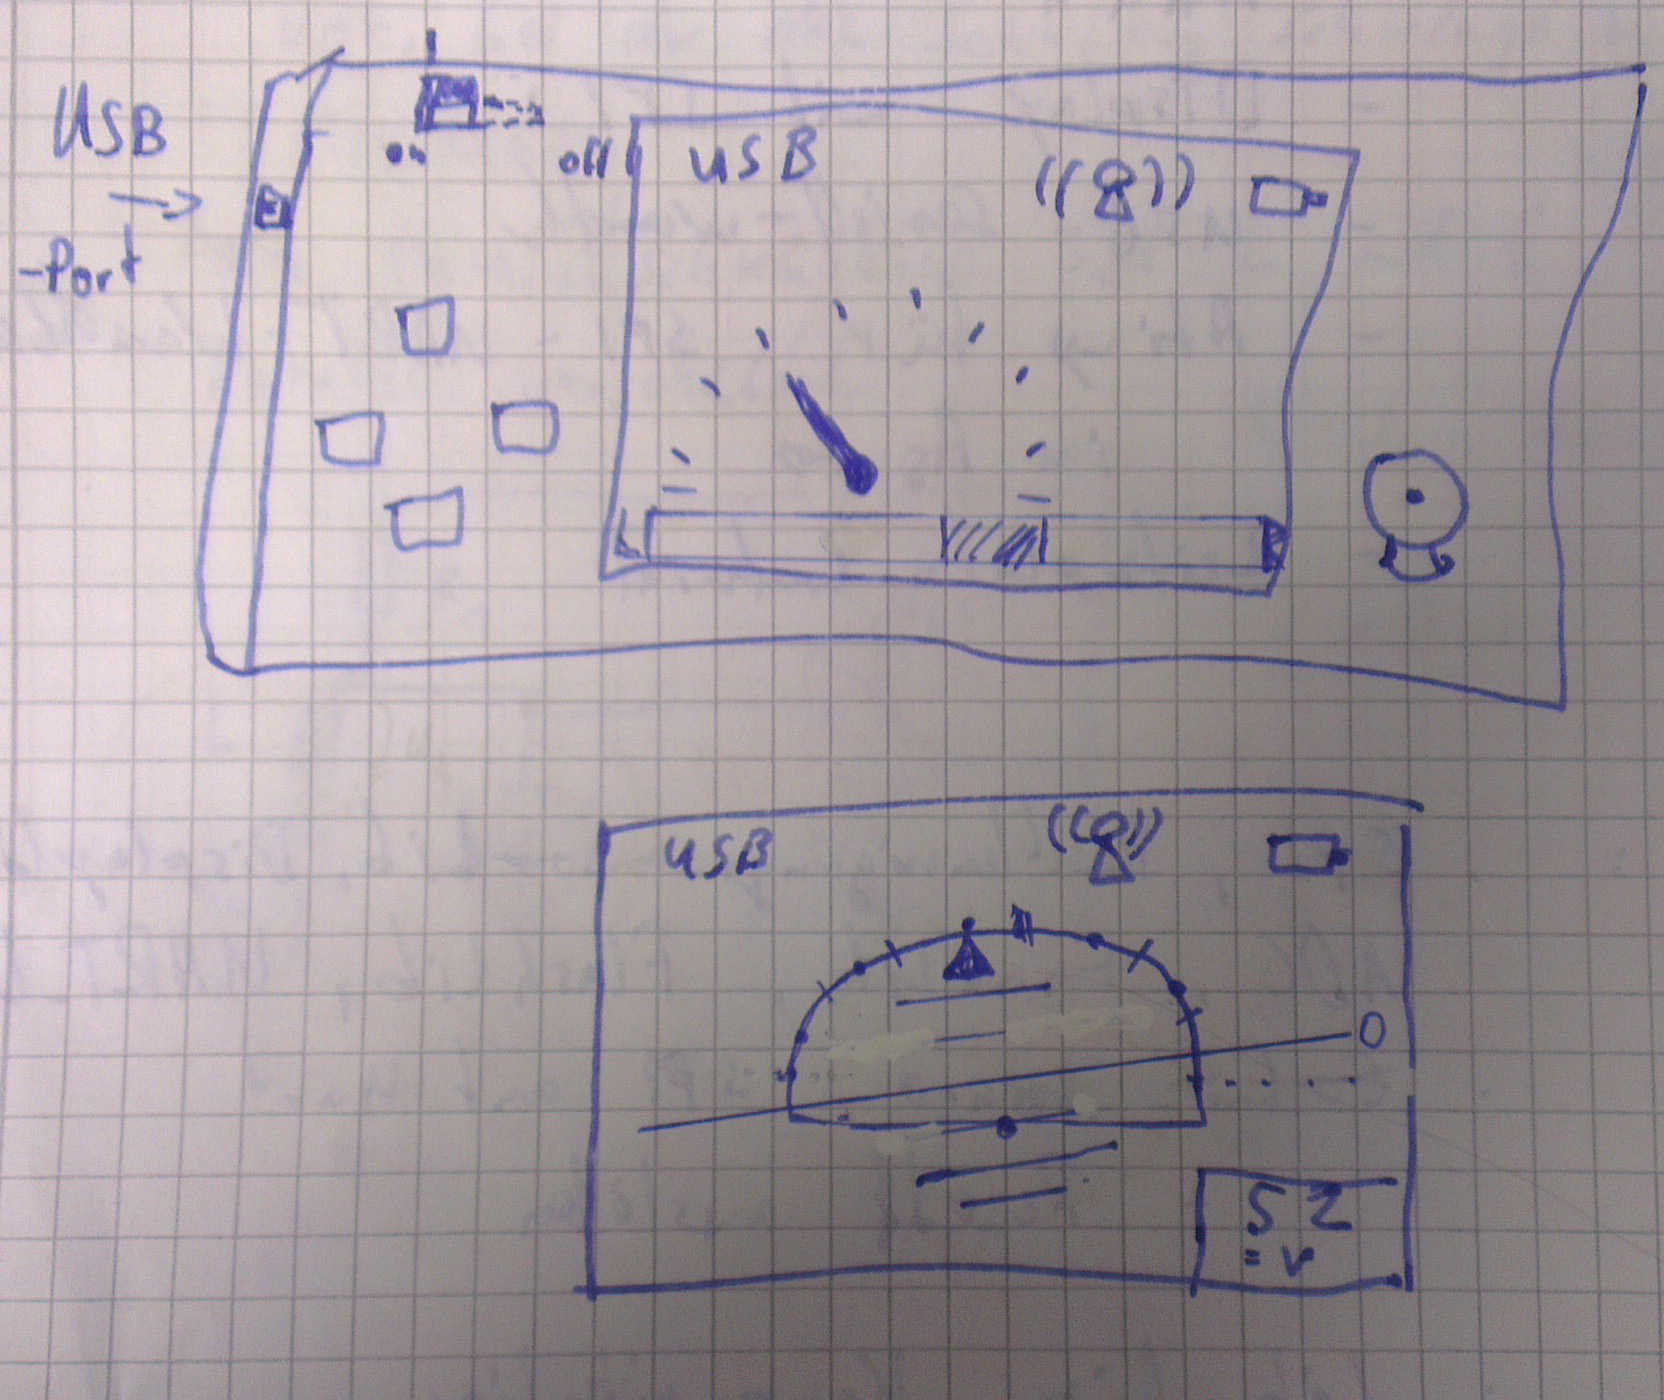
\includegraphics[width=0.7\textwidth]{bilder/idee_controller.jpg}
	\caption{Mögliches Aussehen (Brainstorming)}
	\label{img:idee_controller}
\end{figure}



\chapter{Treffen am 18.12.2014}
\section{Anwesende Personen}
\begin{itemize}
	\item Stefan Biereigel
	\item Rene Winkler
	\item Mathias Fugmann
	\item Junlong Yin
\end{itemize}

\section{Besprochen bzw. Bearbeitet}
Es wurde abschließend zur Entscheidungsmatrix diskutiert und wir kamen zusammen zu dem in \autoref{tab:entscheidung} dargestellten Ergebnis. Bewertet wurde nach dem Schulnotensystem, d.h. "1" ist die beste, "6" die schlechteste Bewertung. Das Konzept mit der niedrigsten Gesamtpunktzahl ist das beste.

\begin{table}[H]
\centering
\begin{tabular}{l|l|l|l}
 				& Blau 	& Grün 	& Rot	\\ \hline
Preis			& 6 	& 1		& 3		\\ \hline
Bedienbarkeit	& 1		& 4		& 2		\\ \hline
Komplexität		& 4		& 2		& 4		\\ \hline
Ähstetik		& 1		& 1		& 3		\\ \hline
Funktionsumfang	& 1		& 4		& 2		\\ \hline
Zuverlässigkeit	& 2		& 2		& 2		\\ \hline
Beschaffbarkeit	& 1		& 1		& 1		\\ \hline \hline
Gesamt			& 16	& 15	& 17	\\ \hline
\end{tabular}
\caption{Entscheidungsmatrix}
\label{tab:entscheidung}
\end{table}

Es zeigte sich schnell, dass die Konzepte alle ungefähr gleich gut abgeschnitten hatten. Jedes Konzept hat seine Vor- und Nachteile, die oft zwischen Preis und Funktionsumfang eintauschbar sind. Wir haben uns daher auf die Entwicklung eines neuen, gesamtheitlichen Konzepts geeinigt. 
Es vereint die preislichen Vorteile in der Übertragungstechnik durch Nutzung der nRF-Funkmodule und den Funktionsumfang (der hauptsächlich durch Software erweitert werden kann) durch Nutzung des Beschleunigungssensor. Es entspricht im wesentlichen dem grünen Konzept mit den eingezeichneten Erweiterungen.
\chapter{Treffen am 05.01.2014}
\section{Anwesende Personen}
\begin{itemize}
	\item Stefan Biereigel
	\item Rene Winkler
	\item Mathias Fugmann
	\item Junlong Yin
\end{itemize}

\section{Besprochen bzw. Bearbeitet}
Rene Winkler hatte entsprechend der am 18.12. besprochenen Pläne zur möglichen Umsetzung eines Konzepts eine Designstudie in Cinema4D angefertigt. Verschiedene Möglichkeiten zur Befestigung der Elektronik im Gehäuse wurden diskutiert.
\begin{itemize}
	\item Verschraubungen von oben (sichtbar) sollten vermieden werden
	\item Verschraubungen von unten sind möglicherweise problematisch
	\item Nach Möglichkeit sollte das Gehäuse in zwei Hälften zerteilbar sein, ohne Kabelverbindungen trennen zu müssen.
	\item Mit produzierte Stehbolzen (Plastik), in welche kleine Plastiktreibschrauben gedreht werden können, können eine gute Möglichkeit sein
\end{itemize}

Die Design-Studie kam bei allen Team-Mitgliedern gut an und lässt eine Abschätzung zur ungefähren Gehäusedimensionen zu.

% Konzepte, erste Version
\begin{figure}
	\centering
	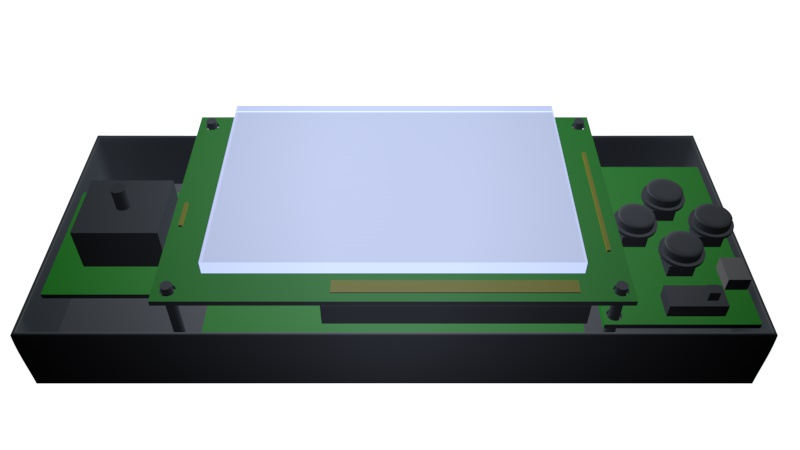
\includegraphics[width=0.7\textwidth]{bilder/studie_controller.jpg}
	\label{fig:designstudie1}
	\caption{Designstudie des Controllers}
\end{figure}

Da Junlong Yin nur noch dieses Semester bei uns ist, wurde mit Herrn Voß für ihn ein Arbeitspaket definiert, welches bis zum Ende des Semesters abzuarbeiten ist: Für die Steuerung über Neigung der Fernbedienung ist eine Weiterverarbeitung der Messwerte aus dem Beschleunigungssensor notwendig. Es wurde folgender Umfang und Ablauf seiner Arbeit definiert:
\begin{itemize}
	\item Analyse der rohen Sensorewerte hinsichtlich Rauschen (Amplitude, Spektrum) relativ zum Nutzsignal (1G in Summe aller Achsen)
	\item Entwicklung eines Modells zur Verbesserung dieser Werte (Filterung, Mittelwert, ...)
	\item Implementierung und Test dieses Modells
	\item Weiterverarbeitung der X-/Y- und Z-Sensorwerte zu Drehwinkeln in allen Achsen (trigonometrische Funktionen), die dann für die Steuerung nutzbar sind.
\end{itemize}
\chapter{Treffen am 12.01.2014}
\section{Anwesende Personen}
\begin{itemize}
	\item Stefan Biereigel
	\item Rene Winkler
	\item Mathias Fugmann
	\item Junlong Yin
\end{itemize}

\section{Besprochen bzw. Bearbeitet}
Stefan und Junlong besprachen das weitere Vorgehen für das abzugebende Arbeitspaket (Messung, Filterung, Auswertung Beschleunigungssensor). Folgendes Vorgehen wurde besprochen:
\begin{itemize}
	\item Inbetriebnahme bestehender Code Beschleunigungssensor - OK
	\item Inbetriebnahme bestehender Code UART (Mit USB-Seriell-Wandler)
	\begin{itemize}
		\item Probleme traten im Zusammenhang mit der Baudrate auf
		\item evtl. ist der Quarz auf dem STM32F4 defekt/out-of-spec?
		\item Versch. Baudraten brachten keine Besserung
		\item Problem: Einzelne Bits sind falsch, teilweise Offset von 0x40 vorhanden
	\end{itemize}
	\item Ausgabe Beschleunigungs-Sensor-Werte auf UART
	\item statistische Auswertung am PC mit Excel, Matlab, etc.
\end{itemize}

Rene und Mathias beschäftigten sich weiter mit der Designstudie für das Gehäuse und besprachen mit Herr Voß verschiedene, evtl. kritische Punkte.
\chapter{Treffen am 15.01.2014}
\section{Anwesende Personen}
\begin{itemize}
	\item Stefan Biereigel
	\item Rene Winkler
	\item Mathias Fugmann
	\item Junlong Yin
\end{itemize}

\section{Besprochen bzw. Bearbeitet}
Rene und Mathias nutzten teilen Teil des Praktikums für die Kommunikation mit dem FB SciTec mit Hinblick auf die Fertigung von Gehäusen.
\begin{itemize}
	\item Herstellung in 3 Verfahren möglich
	\item Aus Kostengründen nur ein Verfahren möglich (FDM, 3D-Druck)
	\item Abschätzung: 10m für ein Gehäuse, 10ct pro Meter etwa
	\item Stärken: 1,5mm Minimum in allen Achsen
	\item STL-Datei als Input für den Druck muss verfügbar sein
	\item Material ist immer verfügbar
	\item Vorlaufzeit: ca. 1 Woche, nicht erst 3 Tage vorher
	\item vorherige Testläufe wären möglich (auch kostenfrei)
	\item Überhänge sind problematisch (bei Design beachten)
\end{itemize}

Weitere Vorschläge und Ideen zum Design wurden besprochen und ausgewertet.

Stefan und Junlong konnten die Probleme am UART des STM32 beheben und erste Messwerte in Excel überführen. Das Problem war, dass in einer der Standard Peripheral Library zugehörigen Dateien noch ein Wert für den Quarz von 25MHz eingetragen war. Nach Hinzufügen der Präprozessordirektive -DHSE\_ VALUE=8000000 war die Baudrate korrekt und die Kommunikation funktionierte.
\chapter{Anhang}

\begin{figure}
	\centering
	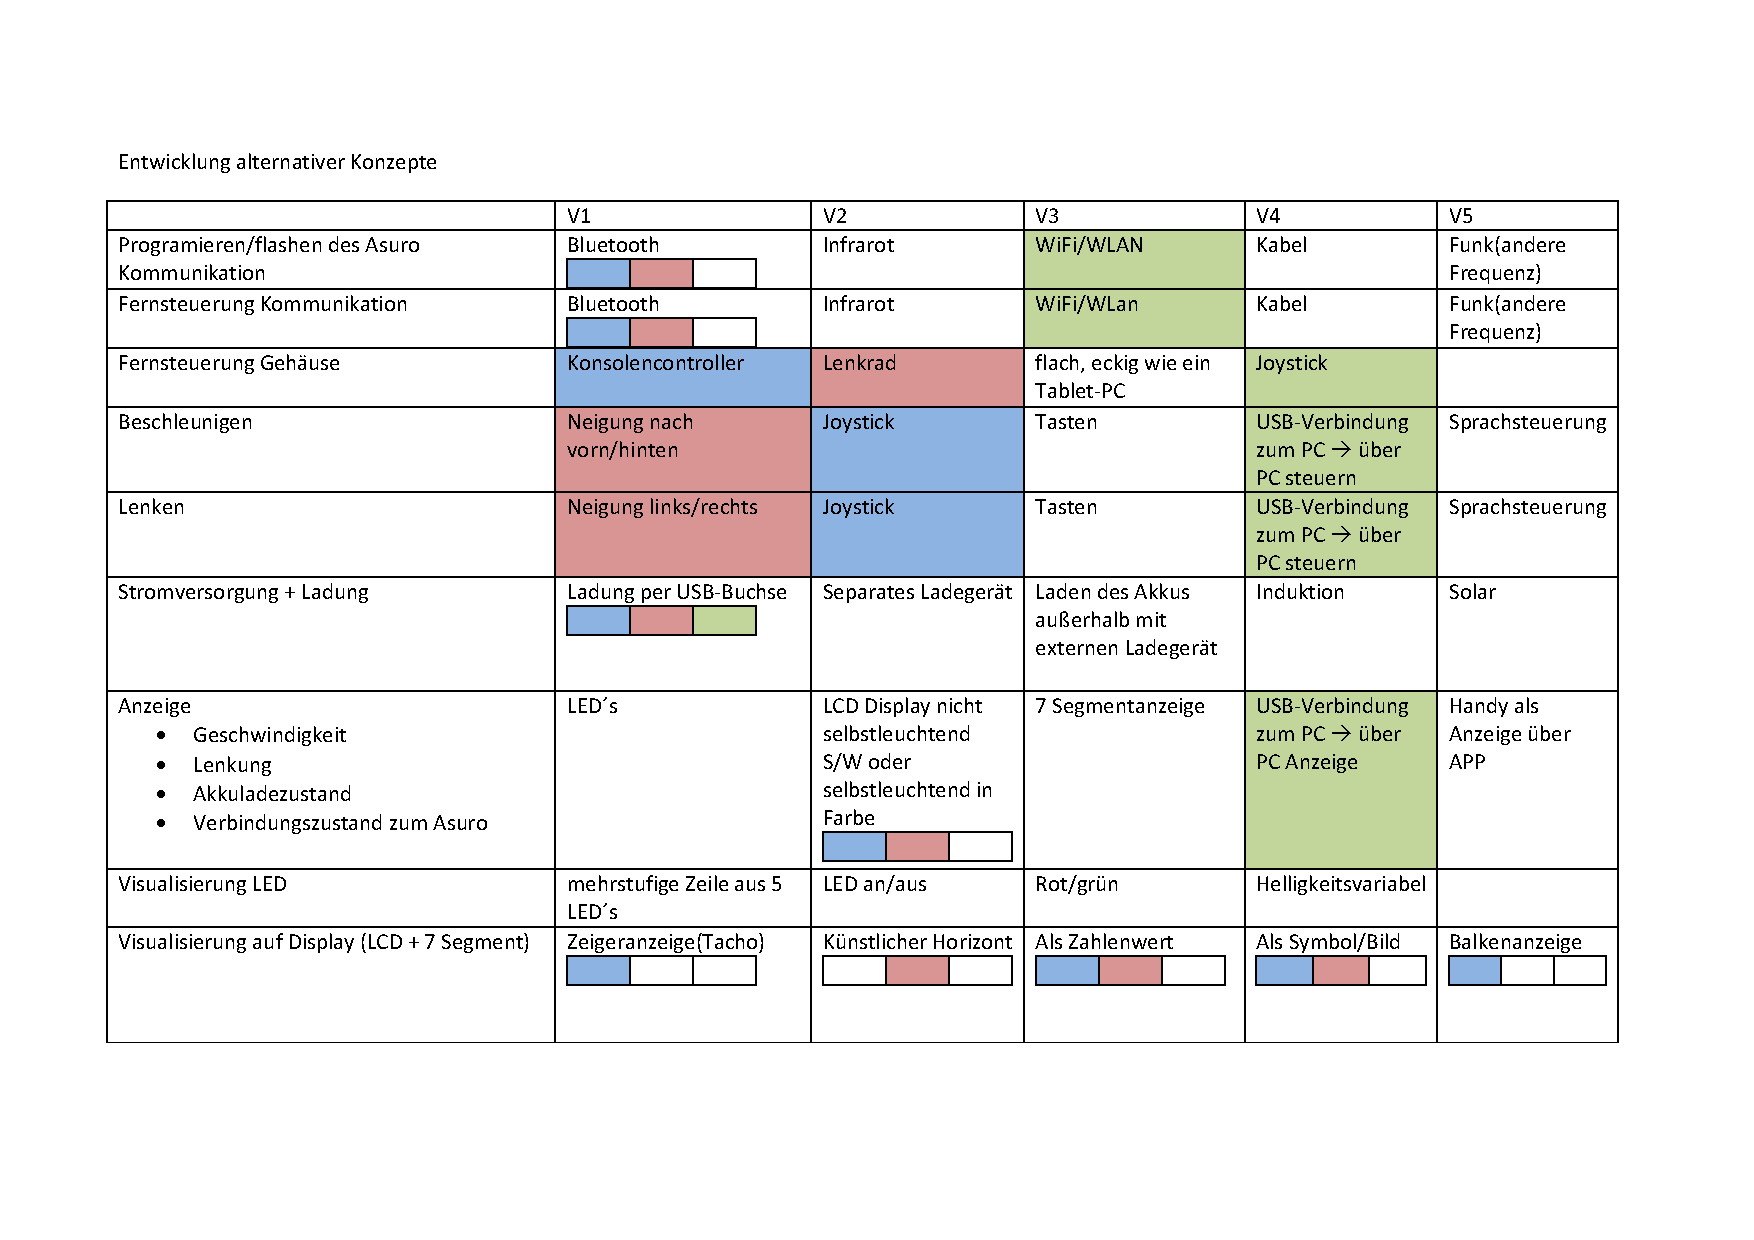
\includegraphics[angle=90, width=\textwidth]{konzepte_v1/Konzepte.pdf}
	\caption{Konzept-Übersicht}
	\label{fig:konzepte}
\end{figure}

% Konzepte, erste Version
\begin{figure}
	\centering
	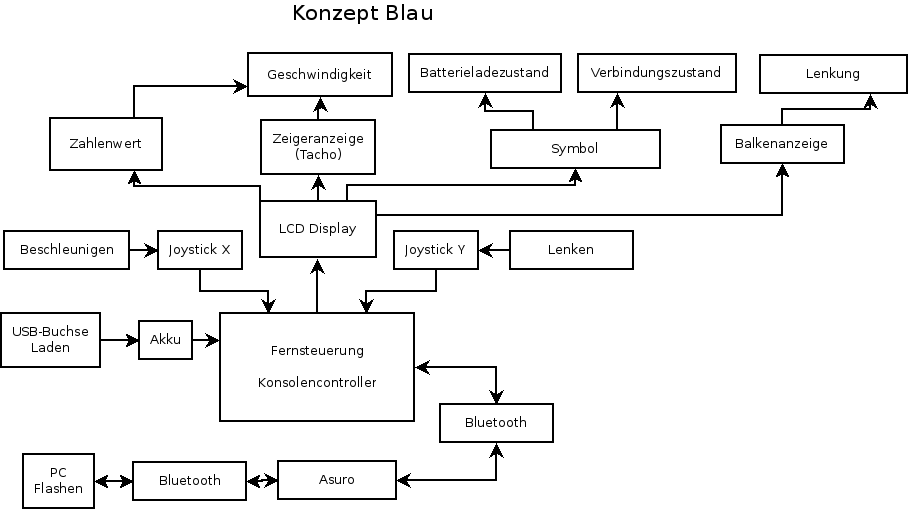
\includegraphics[width=\textwidth]{konzepte_v1/Konzept_Blau.png}
	\label{fig:blau_v1}
	\caption{Konzept Blau, Version 1}
\end{figure}

\begin{figure}
	\centering
	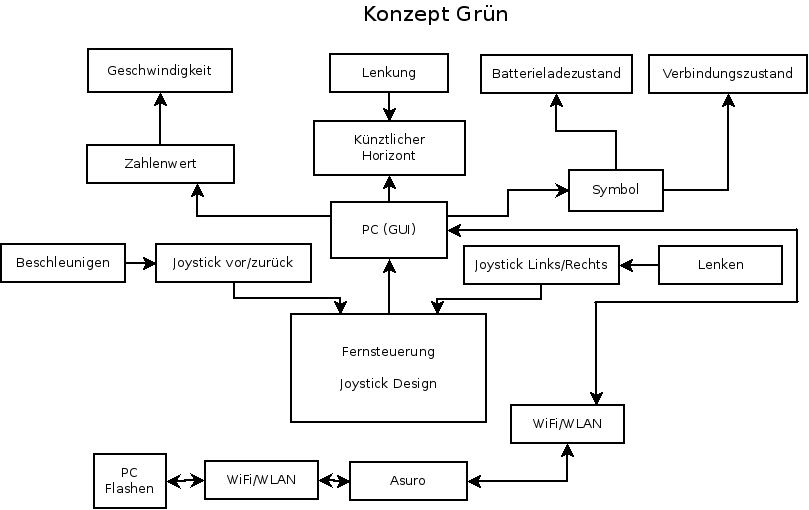
\includegraphics[width=\textwidth]{konzepte_v1/Konzept_Gruen.png}
	\caption{Konzept Grün, Version 1}
	\label{fig:gruen_v1}
\end{figure}

\begin{figure}
	\centering
	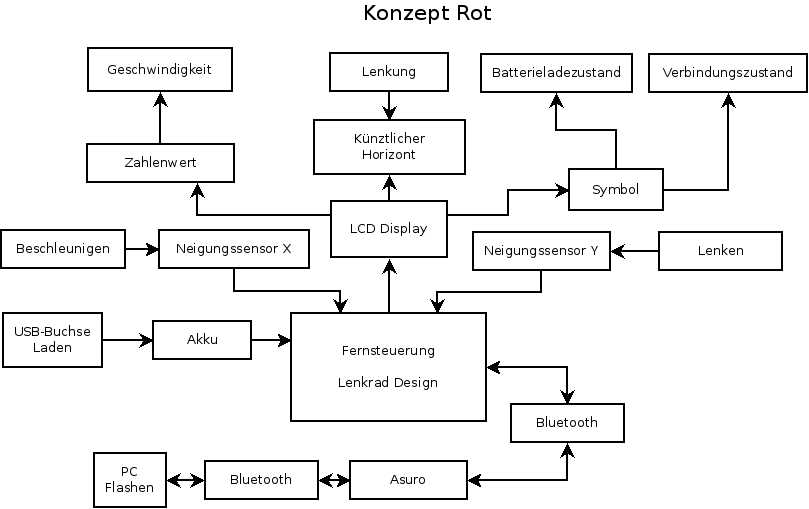
\includegraphics[width=\textwidth]{konzepte_v1/Konzept_Rot.png}
	\caption{Konzept Rot, Version 1}
	\label{fig:rot_v1}
\end{figure}

% Konzepte, zweite Version
\begin{figure}
	\centering
	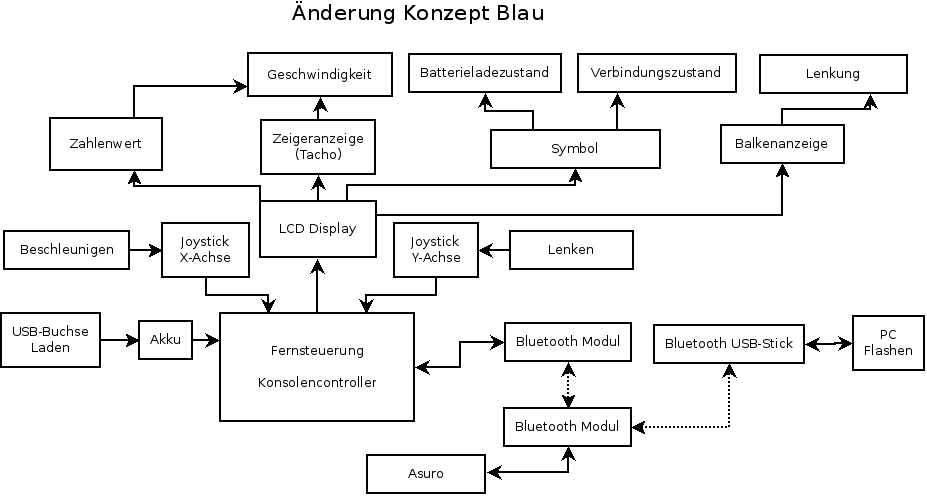
\includegraphics[width=\textwidth]{konzepte_v2/Konzept_Blau.png}
	\caption{Konzept Blau, Version 2}
	\label{fig:blau_v2}
\end{figure}

\begin{figure}
	\centering
	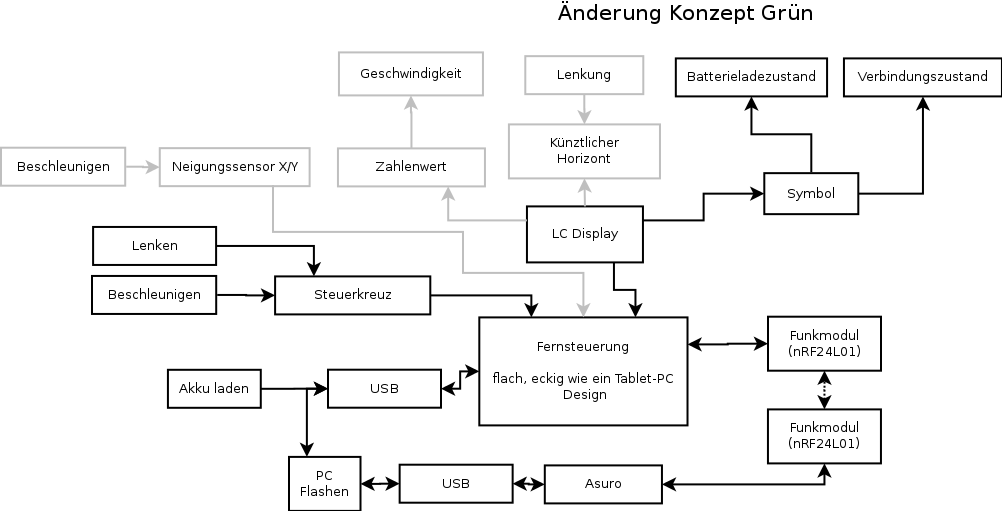
\includegraphics[width=\textwidth]{konzepte_v2/Konzept_Gruen.png}
	\caption{Konzept Grün, Version 2}
	\label{fig:gruen_v2}
\end{figure}

\begin{figure}
	\centering
	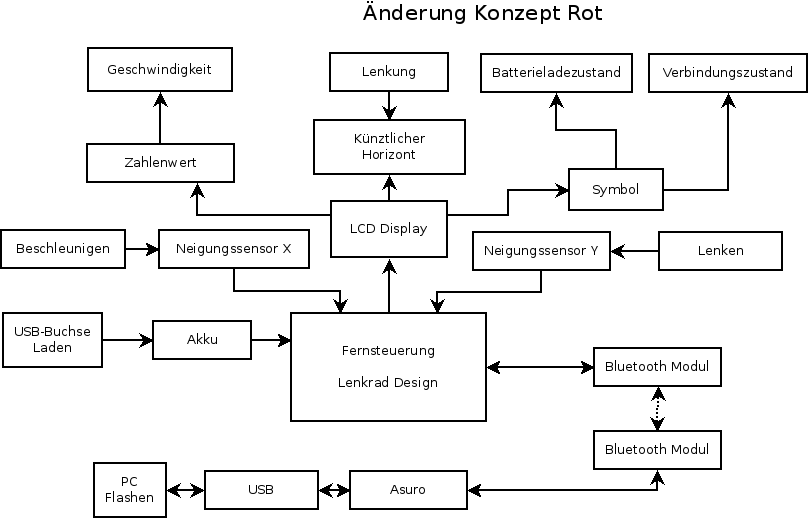
\includegraphics[width=\textwidth]{konzepte_v2/Konzept_Rot.png}
	\caption{Konzept Rot, Version 2}
	\label{fig:rot_v2}
\end{figure}


\listoftables
\listoffigures

\end{document}


